\documentclass[border=14pt]{standalone}
\usepackage{tikz}
\usepackage{amsmath}
\usepackage{amssymb}
\usetikzlibrary{
  arrows.meta,
  calc,
  backgrounds,
  decorations.markings
}

% ============================================================
% Frobenius Mesh 3x3 | Looping Photons | Complex MZI Matrix
%
% Each MZI_{ij}: two beam splitters (blue discs) connected by
% an upper arm (phase path phi_{ij}) and lower arm (amplitude
% path theta_{ij}).  Matrix element: a_{ij} = sin(theta_{ij})
% * exp(i*phi_{ij}).  Three closed photon loops enforce the
% Frobenius closure condition mu o delta = id (IMSCRIB gate).
% ============================================================

\tikzset{
  % Beam splitter node
  bs/.style={
    circle, fill=cyan!45!blue!70, draw=blue!75!cyan,
    line width=0.65pt, minimum size=10pt, inner sep=0pt
  },
  % Phase-ring decoration inside MZI
  ring/.style={
    circle, draw=orange!65!yellow, fill=none,
    line width=0.75pt, minimum size=14pt, inner sep=0pt
  },
  % Amplitude detector/monitor
  det/.style={
    circle, fill=red!55!orange!90, draw=red!75,
    line width=0.5pt, minimum size=7pt, inner sep=0pt
  },
  % Waveguide (main path)
  wg/.style={line width=1.4pt, draw=cyan!40!blue!65},
  % Input / output arrow waveguide
  io/.style={wg, -Stealth},
  % Inter-column connector
  conn/.style={line width=1.1pt, draw=blue!35!cyan!55},
  % Loop paths: row 1 (orange-red), row 2 (amber), row 3 (teal)
  Lp1/.style={line width=1.9pt, draw=orange!90!red,
    postaction={decorate},
    decoration={markings,
      mark=at position 0.58 with {\arrow[scale=1.6, orange!90!red]{Stealth}}}},
  Lp2/.style={line width=1.9pt, draw=yellow!80!orange,
    postaction={decorate},
    decoration={markings,
      mark=at position 0.58 with {\arrow[scale=1.6, yellow!80!orange]{Stealth}}}},
  Lp3/.style={line width=1.9pt, draw=green!55!teal,
    postaction={decorate},
    decoration={markings,
      mark=at position 0.58 with {\arrow[scale=1.6, green!55!teal]{Stealth}}}},
  % Label styles
  milab/.style={font=\footnotesize\bfseries, text=black!50},
  phlab/.style={font=\tiny, text=blue!65!black},
  thlab/.style={font=\tiny, text=red!55!black},
  portlab/.style={font=\small},
  >=Stealth
}

\begin{document}
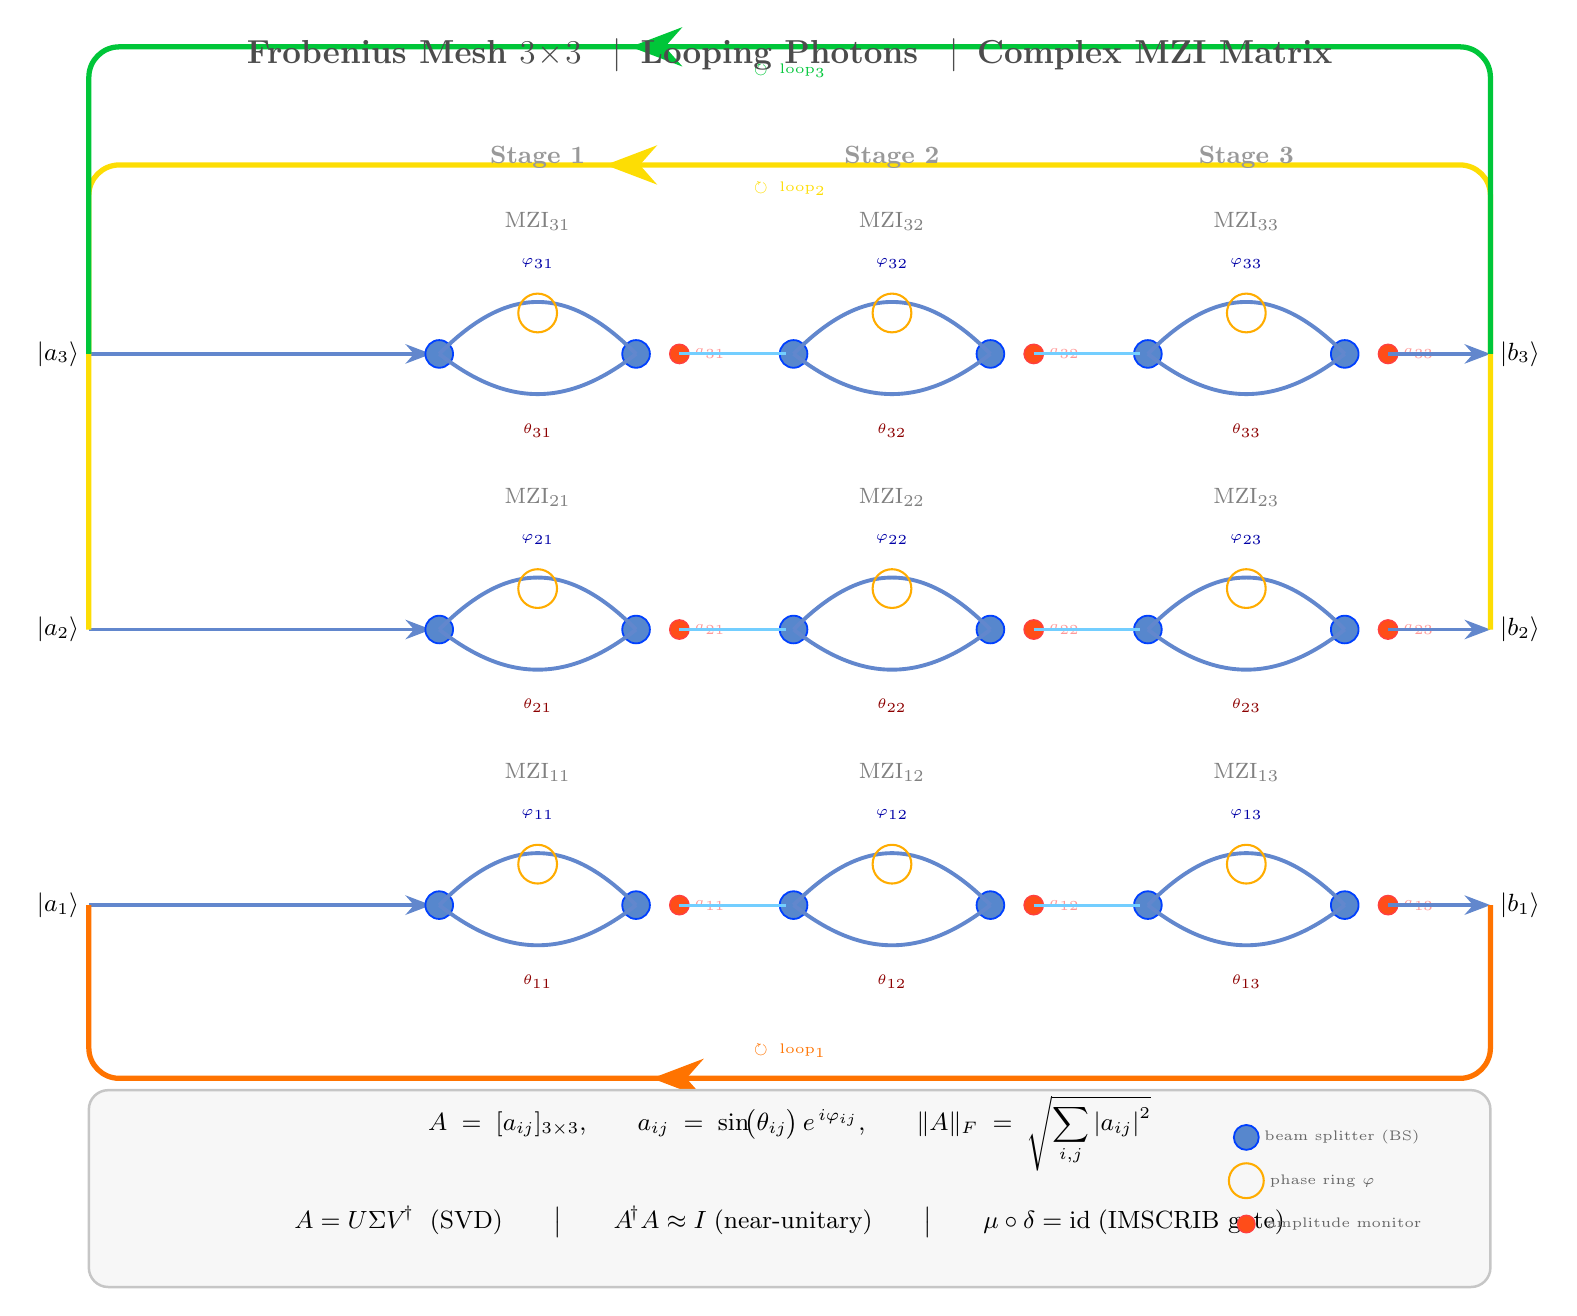
\begin{tikzpicture}[scale=1.0]

% ============================================================
% COORDINATE CONSTANTS
% ============================================================
% Column x-centres (MZI units)
\def\cA{3.5}    % column 1
\def\cB{8.0}    % column 2
\def\cC{12.5}   % column 3
% Row y-positions
\def\rI{0.0}    % row 1  (bottom)
\def\rII{3.5}   % row 2  (middle)
\def\rIII{7.0}  % row 3  (top)
% MZI geometry
\def\hw{1.25}   % BS offset from MZI centre
\def\uarm{0.88} % upper arm Bézier peak above centre
\def\darm{0.68} % lower arm Bézier dip below centre
\def\detoff{0.55}% detector lateral offset past right BS

% ============================================================
% INPUT WAVEGUIDES  (left → first BS)
% ============================================================
\foreach \ry/\lab in {0.0/$\lvert a_1\rangle$, 3.5/$\lvert a_2\rangle$, 7.0/$\lvert a_3\rangle$}{
  \draw[io] (-2.2, \ry) -- (3.5-1.25-0.1, \ry);
  \node[portlab, left] at (-2.2, \ry) {\lab};
}

% ============================================================
% 9 MZI ELEMENTS  (3 rows × 3 columns)
% Each entry: col-x / row-y / row-index / col-index
% ============================================================
\foreach \cx/\cy/\ri/\cj in {
  3.5/0.0/1/1,   8.0/0.0/1/2,   12.5/0.0/1/3,
  3.5/3.5/2/1,   8.0/3.5/2/2,   12.5/3.5/2/3,
  3.5/7.0/3/1,   8.0/7.0/3/2,   12.5/7.0/3/3
}{
  % — Beam splitters —
  \node[bs] at (\cx-1.25, \cy) {};
  \node[bs] at (\cx+1.25, \cy) {};
  % — Upper arm (phase path) —
  \draw[wg] (\cx-1.25, \cy)
      .. controls (\cx-0.38, \cy+0.88) and (\cx+0.38, \cy+0.88) ..
      (\cx+1.25, \cy);
  % — Lower arm (amplitude path) —
  \draw[wg] (\cx-1.25, \cy)
      .. controls (\cx-0.38, \cy-0.68) and (\cx+0.38, \cy-0.68) ..
      (\cx+1.25, \cy);
  % — Phase ring (visual indicator) —
  \node[ring] at (\cx, \cy+0.52) {};
  % — Labels —
  \node[phlab, above] at (\cx, \cy+0.88+0.08) {$\varphi_{\ri\cj}$};
  \node[thlab, below] at (\cx, \cy-0.68-0.08) {$\theta_{\ri\cj}$};
  \node[milab]        at (\cx, \cy+1.68)       {$\mathrm{MZI}_{\ri\cj}$};
  % — Amplitude monitor (detector) —
  \node[det] at (\cx+1.25+0.55, \cy) {};
  % — Matrix element label next to detector —
  \node[font=\tiny, text=red!40, right=2pt] at (\cx+1.25+0.55, \cy)
      {$a_{\ri\cj}$};
}

% ============================================================
% INTER-COLUMN CONNECTORS
% ============================================================
\foreach \ry in {0.0, 3.5, 7.0}{
  % col 1 detector → col 2 left BS
  \draw[conn] (3.5+1.25+0.55, \ry) -- (8.0-1.25-0.1, \ry);
  % col 2 detector → col 3 left BS
  \draw[conn] (8.0+1.25+0.55, \ry) -- (12.5-1.25-0.1, \ry);
}

% ============================================================
% OUTPUT WAVEGUIDES  (col-3 right BS → right label)
% ============================================================
\foreach \ry/\lab in {0.0/$\lvert b_1\rangle$, 3.5/$\lvert b_2\rangle$, 7.0/$\lvert b_3\rangle$}{
  \draw[io] (12.5+1.25+0.55, \ry) -- (15.6, \ry);
  \node[portlab, right] at (15.6, \ry) {\lab};
}

% ============================================================
% CLOSED LOOP PHOTON PATHS  (Frobenius closure: mu o delta = id)
% Each loop exits right, arcs around, re-enters left.
% Arrows placed at 58% of path length (on the return segment).
% ============================================================

% Loop 1 — row 1 — orange-red — BELOW the mesh
\draw[Lp1, rounded corners=11pt]
  (15.6, 0.0) -- (15.6, -2.2) -- (-2.2, -2.2) -- (-2.2, 0.0);
\node[orange!90!red, font=\tiny\bfseries] at (6.7, -1.85)
    {$\circlearrowright\;\mathrm{loop}_1$};

% Loop 2 — row 2 — amber — ABOVE (lower arc)
\draw[Lp2, rounded corners=11pt]
  (15.6, 3.5) -- (15.6, 9.4) -- (-2.2, 9.4) -- (-2.2, 3.5);
\node[yellow!80!orange, font=\tiny\bfseries] at (6.7, 9.1)
    {$\circlearrowright\;\mathrm{loop}_2$};

% Loop 3 — row 3 — teal — ABOVE (higher arc)
\draw[Lp3, rounded corners=11pt]
  (15.6, 7.0) -- (15.6, 10.9) -- (-2.2, 10.9) -- (-2.2, 7.0);
\node[green!55!teal, font=\tiny\bfseries] at (6.7, 10.6)
    {$\circlearrowright\;\mathrm{loop}_3$};

% ============================================================
% COLUMN HEADER LABELS
% ============================================================
\node[font=\small\bfseries, text=black!40] at (3.5,  7.0+2.5) {Stage 1};
\node[font=\small\bfseries, text=black!40] at (8.0,  7.0+2.5) {Stage 2};
\node[font=\small\bfseries, text=black!40] at (12.5, 7.0+2.5) {Stage 3};

% ============================================================
% TITLE
% ============================================================
\node[font=\large\bfseries, align=center, text=black!70]
    at (6.7, 7.0+3.8) {Frobenius Mesh $3\!\times\!3$ \enspace$|$\enspace
    Looping Photons \enspace$|$\enspace Complex MZI Matrix};

% ============================================================
% LEGEND / ANNOTATION BOX  (below the diagram)
% ============================================================
\begin{scope}[shift={(0, -3.5)}]
  \draw[rounded corners=7pt, draw=gray!45, fill=gray!6, line width=0.9pt]
      (-2.2, -1.35) rectangle (15.6, 1.15);

  % Row 1: matrix and element formula
  \node[font=\small, align=center] at (6.7, 0.60) {%
    $A \;=\; [a_{ij}]_{3\times3}$,\qquad
    $a_{ij} \;=\; \sin\!\bigl(\theta_{ij}\bigr)\,
      e^{\,i\varphi_{ij}}$,\qquad
    $\|A\|_F \;=\; \sqrt{\displaystyle\sum_{i,j}|a_{ij}|^2}$%
  };

  % Row 2: SVD, unitarity, Frobenius identity
  \node[font=\small, align=center] at (6.7, -0.52) {%
    $A = U\Sigma V^{\!\dagger}$ \;(SVD)\qquad$\big|$\qquad
    $A^{\!\dagger}A \approx I$\;(near-unitary)\qquad$\big|$\qquad
    $\mu\circ\delta = \mathrm{id}$\;(IMSCRIB gate)%
  };
\end{scope}

% ============================================================
% LEGEND ICONS  (bottom-right corner)
% ============================================================
\begin{scope}[shift={(12.5, -3.5)}]
  \node[bs, scale=0.9] at (0, 0.55) {};
  \node[font=\tiny, right=3pt, text=black!60] at (0, 0.55) {beam splitter (BS)};
  \node[ring, scale=0.9] at (0, 0.0) {};
  \node[font=\tiny, right=5pt, text=black!60] at (0, 0.0) {phase ring $\varphi$};
  \node[det, scale=0.9] at (0, -0.55) {};
  \node[font=\tiny, right=4pt, text=black!60] at (0, -0.55) {amplitude monitor};
\end{scope}

\end{tikzpicture}
\end{document}
